\chapter{The Core Execution Environment}
\label{cee-chapter}

This chapter describes the core execution environment (CEE) of an
SCJVM, which executes Java bytecode instructions.
The CEE is aware of the structure of Java objects and classes in order
to handle bytecode instructions properly.
In addition, the CEE of an SCJVM manages the flow of execution
dictated by the SCJ programming model, including, for example, safelet
setup and mission execution.

As shown in Figure~\ref{cee-fig}, we view the core execution
environment as having three components:
\begin{itemize}
\item the object manager, which manages information about objects
  created during execution of the bytecode,
\item the interpreter, which handles execution of bytecode
  instructions, and
\item the launcher, which coordinates the startup of the SCJVM, the
  execution of missions, and the execution of methods in the
  interpreter.
\end{itemize}
The interpreter is central to the main functionality of the core
execution environment, but proper handling of infrastructure methods
requires handling the SCJ mission-based programming model, which is
dealt with by the launcher.
The interpreter requires access to memory, but the class information
and bytecode instructions do not change throughout the execution of
the SCJVM, so they are provided as global constants in our model that
are passed to the interpreter as parameters.
Objects do change throughout the execution of the SCJVM and are in a
separate region of memory to classes and bytecode instructions.
The management of objects is handled by the object manager component
of the core execution environment.

\begin{figure}[ht]
  \centering
  \begin{tikzpicture}

    \coordinate (width)  at (10cm,0cm);
    \coordinate (height) at (0cm,6cm);

    \path (0,0) -- (height)
    coordinate[pos=0.18] (OS boundary)
    coordinate[pos=0.20] (VM part bottom)
    coordinate[pos=0.57] (VM part top)
    coordinate[pos=0.60] (API boundary)
    coordinate[pos=0.82] (App boundary);
    
    \path (VM part bottom) -- (VM part top)
    coordinate[pos=0.7] (CEE part top);

    \path (VM part bottom) -- (VM part top)
    coordinate[pos=0.85] (CEE ypos);

    \path (0,0) -- (width)
    coordinate[pos=0.04] (CEE left)
    coordinate[pos=0.76] (CEE right)
    coordinate[pos=0.78] (VM Services left)
    coordinate[pos=0.96] (VM Services right)
    coordinate[pos=0.01] (CEE part sep);

    \path (CEE left) -- (CEE right)
    coordinate[pos=0.5] (CEE xpos);

    \path (0,0) to node[pos=0.5] (mid) {} (width);
    \path (0,0) to node[pos=0.25] (quart) {} (width);

    \draw (0,0) rectangle (width |- height);

    \draw (OS boundary) -- ++(width);
    \path (0,0) rectangle node[pos=0.5] (OS) {} (width |- OS boundary);
    \draw (mid |- API boundary) rectangle node[pos=0.5] (API) {} (width |- App boundary);
    \draw (App boundary) -- ++(width);
    \path (App boundary) rectangle node[pos=0.5] (App) {} (width |- height);

    \path (quart |- API boundary) rectangle node[pos=0.4] (SCJVM) {} (quart |- App boundary);
    \draw (CEE left |- VM part bottom) rectangle (CEE right |- VM part top);
    \draw (VM Services left |- VM part bottom) rectangle node[pos=0.5] (VM Services) {} (VM Services right |- VM part top);
    \coordinate (CEE) at (CEE xpos |- CEE ypos);

    \node[align=center] at (App)   {SCJ Application};
    \node[align=center] at (API)   {SCJ\\Infrastructure\\and API};
    \node[align=center] at (SCJVM) {SCJ\\Virtual Machine};
    \node[align=center] at (CEE)   {Core Execution Environment};
    \node[align=center] at (VM Services)  {SCJVM\\Services};
    \node[align=center] at (OS)    {Operating System/Hardware Abstraction Layer};

    \foreach \x in {1,...,3}
    \pgfmathsetmacro{\a}{0.33*(\x - 1)}
    \pgfmathsetmacro{\b}{0.33*\x}
    \path ($(CEE left) + (VM part bottom)!0.07!(VM part top)$) -- 
    node[pos=\a] (CEE part \x start) {}
    node[pos=\b] (CEE part \x end) {}
    ($(CEE right) + (VM part bottom)!0.07!(VM part top) - (CEE part sep)$);

    \foreach \x in {1,...,3} 
    \draw ($(CEE part \x start) + (CEE part sep)$)
    rectangle node[pos=0.5] (CEE part \x) {}
    (CEE part \x end |- CEE part top);
    
    \node[align=center] at (CEE part 1) {\small Object \\ \small Manager};
    \node[align=center] at (CEE part 2) {\small Interpreter};
    \node[align=center] at (CEE part 3) {\small Launcher};
  \end{tikzpicture}
  \caption{Structure of an SCJVM and its relation to the SCJ
    infrastructure and the operating system/hardware abstraction
    layer}
  \label{cee-fig}
\end{figure}

The CEE is combined with the SCJVM services to form the complete
SCJVM; this can be seen in Figure~\ref{cee-fig}, which shows the same
structure described in Figure~\ref{scjvm-services-fig} in the previous
chapter, but has a focus on the CEE components.
The CEE is the starting point for our compilation strategy, which is
another main component of our framework for verification of SCJVMs,
the SCJVM services are unaffected by the compilation strategy and can
be implemented a separate library.

Each of the components of the CEE is represented by a single \Circus{}
process in our model.
The structure of the communication between the processes is show in
Figure~\ref{cee-model-fig}.
The memory is used by the interpreter and launcher to create objects
and enter backing stores.
The memory then communicates the memory manager described in the previous
chapter to allocate memory for objects and clear backing stores.
The launcher also communicates with the memory manager to allocate
backing stores and handle calls to SCJVM memory manager services.
It must also communicate with the scheduler for the same reason.
The launcher and interpreter communicate with each other as the
launcher executes methods in the interpreter and the interpreter
passes special method invocations back to the launcher for handling.
Finally, the scheduler, in addition to accepting calls to its services
from the launcher, informs the interpreter and memory when a thread is
started, removed or switched to, so that thread switches can be
properly handled.

\begin{figure}[ht]
  \centering
  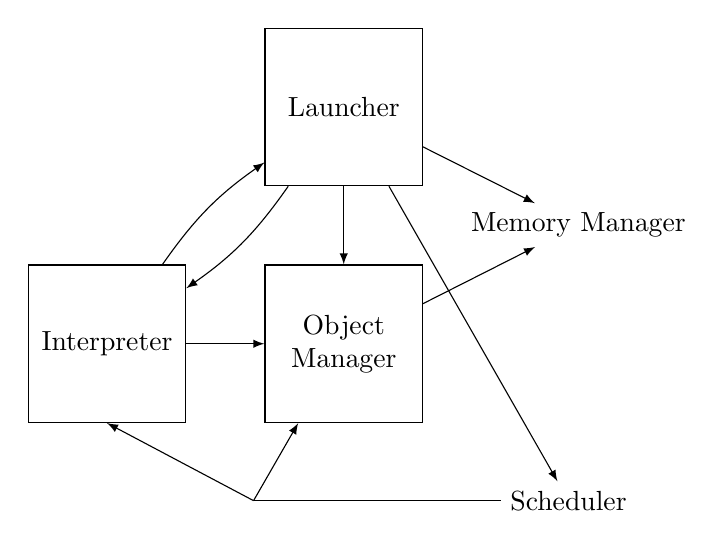
\begin{tikzpicture}
    \node[draw, minimum size = 2cm, below right=2cm, align=center]       (M) {Object\\Manager};
    \node[draw, minimum size = 2cm, below=2cm]       (I) {Interpreter};
    \node[draw, minimum size = 2cm, right=2cm] (L) {Launcher};

    \draw[-latex, bend left=10] (I) edge (L);
    \draw[-latex, bend left=10]  (L) edge (I);
    \draw[-latex] (I) edge (M);
    \draw[-latex] (L) edge (M);
    

    \node[below=1.5cm, right=4.5cm] (MM) {Memory Manager};
    \node[below=5cm, right=5cm] (S) {Scheduler};
    \draw[-latex] (M) edge (MM);
    \draw (S) -- +(-4,0) coordinate (X);
    \draw (X) edge[-latex] (M);
    \draw (X) edge[-latex] (node cs:name=I, anchor=south);
    \draw (L) edge[-latex] (S);
    \draw (L) edge[-latex] (MM);
  \end{tikzpicture}
  \caption{The processes in the core execution environment model and
    their communcation with the each other and the SCJVM services}
  \label{cee-model-fig}
\end{figure}

This chapter begins in Section~\ref{cee-assumptions-section} with an
explanation of the bytecode subset used in our work.
Afterwards, each part of the \Circus{} model of the core execution
environment is presented in a separate section.
The object manager, along with the structure of objects, is
described in Section~\ref{cee-memory-section}.
The interpreter is described by first describing the stack frame
structure in Section~\ref{cee-stack-frames-section}, then the
interpreter itself is presented in
Section~\ref{cee-interpreter-section}.
The launcher is presented in Section~\ref{cee-launcher-section}.
Finally the parts are drawn together into the complete model in
Section~\ref{complete-cee-section}. 
A full version of the CEE model can be found in
Appendix~\ref{full-cee-model}.

\section{Bytecode Subset}
\label{cee-assumptions-section}

Due to the complexity of the JVM and Java bytecode, we model a subset
of Java bytecode.
It is sufficient to express a wide variety of SCJ programs and
illustrate how further features may be added, but small enough to
permit effective reasoning.
The subset has been chosen by considering the bytecode generated from
a minimal SCJ program and removing instructions similar to those
already in the subset.
This ensures the model is not unnecessarily complicated with trivial
or redundant instructions, so we can concentrate on the instructions
that are most of interest in creating the compilation strategy.

The bytecode instructions in our subset are described in
Table~\ref{bytecode-subset-table}.
Java bytecode instructions operate over a state that records
information on all loaded classes, a stack frame, and the object data
residing in memory.
Various pieces of class information are required for execution of
bytecode instructions, but a constant pool, which stores all the
constants and names required by the class, is the main information
used.
The constant pool contains references to classes, methods and fields
used by the bytecode instructions in the class, as well as constant
values used in the code.
The form of the constant pool is a large array.
Indices into this array are used as parameters to instructions
requiring information from the constant pool.
For example, the \texttt{getfield} and \texttt{putfield} instructions
take constant pool index parameters pointing to a reference to a field
whose value should be obtained or set.
Other class information used at runtime includes information on fields
and methods belonging to the class, which is required for creation of
objects and invocation of methods.

\begin{table}
  \centering
  \begin{tabular}{llp{8cm}}
    \hline
    Instruction & Parameter & Description \\
    \hline
    \texttt{aconst\_null} & (none) & 
    Pushes a null object reference onto the operand stack.
    \\
    \texttt{aload} & local variable index &
    Loads the value from a specified local variable and pushes it
    onto the operand stack.
    \\
    \texttt{areturn} & (none) &
    Returns from the current method, pushing the value on top of the
    current method's operand stack onto the operand stack of the
    method returned to.
    \\
    \texttt{astore} & local variable index &
    Pops a value from the operand stack and stores it in the specified
    local variable.
    \\
    \texttt{dup} & (none) &
    Duplicates the value on top of the operand stack.
    \\
    \texttt{getfield} & constant pool index &
    Pops an object reference from the operand stack, gets the value of
    the field specified by the identifier at the given constant pool
    index for the referenced object, and pushes it onto the operand
    stack.
    \\
    \texttt{iadd} & (none) &
    Pops two integer values from the operand stack, adds them, and
    pushes the result back onto the operand stack.
    \\
    \texttt{iconst} & integer value &
    Pushes the given integer value onto the operand stack of the
    current method.
    \\
    \texttt{ineg} & (none) &
    Pops an integer value from the operand stack, negates it, and
    pushes the negated value onto the operand stack.
    \\
    \texttt{invokespecial} & constant pool index &
    Gets the method and class identifier at the given constant pool
    index and invokes the specified method of the specified class,
    popping the method's arguments, including a \texttt{this} object
    reference, from the operand stack.
    \\
    \texttt{invokevirtual} & constant pool index &
    Gets the method and class identifier at the given constant pool
    index, pops the arguments of the specified method, including a
    \texttt{this} object reference, from the operand stack, and
    invokes the specified method of the class of referenced object.
    \\
    \texttt{new} & constant pool index &
    Allocates a new object of the class specified by the identifier at
    the given constant pool index and pushes a reference to the new
    object onto the operand stack.
    \\
    \texttt{putfield} & constant pool index &
    Pops an object reference and value from the operand stack and
    stores the value in the field specified by the identifier at the
    given constant pool index for the referenced object.
    \\
    \texttt{return} & (none) &
    Returns from a method with no return value.
    \\
    \hline
  \end{tabular}
  \caption{The instructions in our bytecode subset}
  \label{bytecode-subset-table}
\end{table}

The frame stack forms the second part of the JVM manipulated by
bytecode instructions and consists of a series of frames that contain
the runtime information for each invocation of a method.
When a method is invoked, a new stack frame is created for it and
pushed onto the frame stack, and when the method returns, the stack
frame is popped from the stack.
Each stack frame contains an operand stack, which is used to store
values manipulated by bytecode instructions, and an array of local
variables.
Most bytecode instructions manipulate the operand stack in some way,
popping arguments from it, pushing results to it or performing
specific operations upon it (such as in the case of the \texttt{dup}
instruction, which duplicates the value on top of the operand stack).
The local variables are used to store the arguments of a method and
the results of computations performed on the operand stack.
Operations are not performed directly on the local variables, so the
only bytecode instructions that affect them are those for moving
values between the operand stack and the local variables
(\texttt{aload} and \texttt{astore} are examples of such
instructions).

Some bytecode instructions also manipulate objects, which in our case
reside in backing store memory.
Such instructions include \texttt{new}, which creates objects, and
\texttt{getfield}, which gets the value from a field of an object.

In our choice of instructions for the subset, we mainly focus on
manipulation of objects and method invocation, since those are core
concepts of Java bytecode and require special handling by the
compilation strategy.

The instruction \texttt{dup} is included as an example of a simple
instruction that operates on the operand stack.
It has been chosen for its frequent occurrence in object initialisation.
Other instructions that do simple operand stack manipulation,
including the arithmetic instructions, can be specified similarly.

Instructions that create object references and pass them around are
also included to allow the full range of object manipulations.
However, arrays are not included as they require additional
instructions and can be emulated, albeit inefficiently, with the
instructions given here.

Both the \texttt{invokevirtual} and \texttt{invokespecial}
instructions, which invoke methods on objects, are included.
The \texttt{invokevirtual} instruction looks up the method to invoke
in the method table for the class of the object that the method is
invoked on.
The \texttt{invokespecial} method, on the other hand, uses the class
identifier supplied in the method reference pointed to by the
parameter of the instruction when looking up the method.

We do not handle exceptions; errors in the SCJVM are instead handled
by simply aborting execution.
While the exception handling mechanism of Java is quite complex, the
correct application of formal methods should eliminate errors in the
SCJVM.
The bytecode instructions that relate to throwing and catching
exceptions are, therefore, not included in our bytecode subset.

As a simplifying assumption, we consider that all values consist of
only a single virtual machine word.
This means that \texttt{long} and \texttt{double} values are not
handled.
Any SCJ API methods that take \texttt{long} or \texttt{double}
arguments are viewed as taking \texttt{int} or \texttt{float} instead.
The reason for this assumption is that handling of two word values
complicates many bytecode instructions while adding little to the
power of the bytecode subset.
This makes little difference at the level of the formal model and our
approach can be easily extended to deal with more types.

Further, we do not make a distinction between the different virtual
machine types in our bytecode instructions.
This is justified as the bytecode instructions simply handle values as
32-bit words, with the type information only used for typechecking
during bytecode validation, which the code passed into the core
execution environment can be assumed to have already passed (it may be
done by a separate component, which can be made safe using existing
work on bytecode validation~\cite{klein2003, stark2001, coglio2000,
  xavier2003}). 
Instead, we include instructions that handle values as object
references, since many of the instructions behave the same for
different types.
We would introduce a lot of duplication in the model if, for example,
both the \texttt{areturn} and \texttt{ireturn} instructions were to be
included.

We also include a few arithmetic instructions as an example of how
integers would be handled.
Specifically, we include the integer addition operation,
\texttt{iadd}, as an example of a binary operation, and the integer
negation operation, \texttt{ineg}, as an example of an unary
operation.
We do not include operations for floating point values since the
operations upon them are not substantially different from those on
integers at the level of modelling and compilation.
The model can be easily extended to include more integer operations.

We also do not consider static methods and fields.
That would add some complexity to our model and most of the
considerations are covered by non-static methods and fields.

Because we are considering bytecode arising from an SCJ program, some
requirements of SCJ permit further simplifications to our bytecode
subset.
The \texttt{invokedynamic} instruction performs method invocation with
runtime typechecking, mainly for the purpose of implementing
dynamically-typed languages targeting the JVM (though it is also used
to implement the lambda expressions introduced in Java 8).
It is not included in our subset as it does not allow static
typechecking and so should not be used for SCJ.

The requirement for all classes to be loaded at startup greatly
simplifies the semantics of several instructions since dynamic class
loading does not need to be considered.
It also means that method lookup tables can be precomputed, which
simplifies method lookup.
This means that the semantics of the \texttt{invokevirtual} and
\texttt{invokeinterface} instructions are the same, since they both
invoke a method on an object, using the object's class as the class
for method lookup.
They, therefore, do not both need to be included and so we have not
included the \texttt{invokeinterface} instruction, since it exists
only to optimise method lookup.

In terms of concurrency considerations, we are assuming our SCJVM to
be single processor, and so we do not need to have more than one
interpreter.
We also assume that thread switches can only occur between bytecode
instructions in the interpreter.
This is justified since bytecode instructions should be atomic.
Execution occurring in other parts of the core execution environment
can also be made atomic via disabling of interrupts.
This is advisable since such execution often involves manipulation of
shared state.

We also do not consider the SCJ mission termination protocol since it
is complex and is not relevant to the central focus of the model,
which is the handling of bytecode instructions.

Having described our bytecode subset and the assumptions we are
making, we now present our model of the core execution environment,
beginning with an explanation of the class structure in the next
section.

\section{Classes}
\label{cee-classes-section}

This section discusses the representation in our model of the
information in Java class files.
We identify the information that is relevant to our bytecode subset
and present a Z schema to represent the class information needed by
the SCJVM at runtime.
The class type is used in the definition of the class information that
is passed to the object manager and the interpreter.

\input{../../SCJ-VM/James/classes.zed}

\section{Object Manager}
\label{cee-memory-section}

The SCJVM memory manager deals with memory solely in terms of sets of
memory addresses, meaning that it the core execution environment needs
to manage objects itself.
As objects are used throughout the core execution environment, in both
the interpreter and launcher, the management of objects is handled in
a separate \Circus{} process, which is described in this section.

\input{../../SCJ-VM/James/memory.zed}

\section{Stack Frames}
\label{cee-stack-frames-section}

The JVM has a stack composed of a series of stack frames, which
contain information about the invoked methods.
The representation of stack frames is described in this section as
stack frames are, like classes, a large data type of interest as a
significant part of the JVM state.
The stack frames are used to form the frame stack used by the
interpreter in the next section.

\input{../../SCJ-VM/James/stack_frames.zed}

\section{Interpreter}
\label{cee-interpreter-section}

The interpreter manages the execution of the bytecode instructions of
methods.
This includes handling the frame stack and program counter, as well as
processing the bytecode instructions themselves according to their
semantics.
The interpreter must also handle thread switches, maintaining an
interpreter state for each thread, since thread switches may occur
between bytecode instructions.

\input{../../SCJ-VM/James/interpreter.zed}

\section{Launcher}
\label{cee-launcher-section}

The launcher is the component of the core execution environment
that coordinates the execution of bytecode instructions by
the interpreter and manages parts of the SCJ infrastructure such as
the safelet and mission model.

\input{../../SCJ-VM/James/launcher.zed}

\section{Complete Core Execution Environment Model}
\label{complete-cee-section}

We now combine the four \Circus{} processes representing the different
components of the core execution environment into a single \Circus{}
process representing the entire core execution environment.

\input{../../SCJ-VM/James/complete_cee.zed}

\section{Final Considerations}
\label{cee-final-considerations-section}

In this chapter we have presented our model of the core execution
environment (CEE) of an SCJVM and specified the subset of Java
bytecode covered in our model.
Our bytecode subset consists of 14 instructions, which focus on method
invocation and the manipulation of objects, since those are core
concepts of Java.
We have omitted instructions for exception handling, since that would
compilicate the model while adding little power.
Our subset is sufficiently small to permit reasoning, but large enough
to express a variety of SCJ programs.

Our CEE model is divided in three components, with a \Circus{} process
representing each component.
The first component is the memory, which manages objects and the
entering of backing stores, since the memory manager discussed in the
previous chapter has no knowledge of the structure of objects.
The second component of the CEE model is the interpreter, which
describes the semantics of each of the bytecode instructions in our
subset and provides for executing methods.
The third and final component is the interpreter, which manages the
SCJ mission model and coordinates execution.

One interesting point about our model is the handling of special
methods in the interpreter and launcher.
This is necessary for several reasons: to allow methods running in the
interpreter to access the SCJVM services defined in the previous
chapter, to allow mission setup methods to interact with the launcher,
and to permit entering of memory areas by interaction with the CEE
memory component.
The handling of special methods works by having the interpreter check
upon invocation of a method whether it requires special handling.
If it does require special handling, it is passed to the launcher to
be handled.
The launcher then performs the required handling of the method,
communicating with the SCJVM services and the memory as required.

This model forms the first part of our compilation strategy, which is
the specification of the source language.
That is mostly included in the interpreter section as the semantics of
the bytecode instructions, though handling of special methods passed
to the launcher and the representation of classes and objects must
also be considered in the compilation strategy.
There are also other possible uses for the model presented in this
chapter.
Since it is a model of an interpreting SCJVM, it could be used as a
specification for an implementation of an interpreting SCJVM.
Such an SCJVM could also incorporate the compilation strategy to
provide a choice between interpreted and complied code, as in the
icecap HVM.
Additionally, since error handling in our model is done via aborting
execution, an identification of the conditions required for the model
to be divergence-free would produce requirements that can be used for
bytecode verification.
